\icode{N23J-MV-SI-L2-261011-002}
\nceeID[3]{2023北京}{4}
位于坐标原点处的波源发出一列沿\(x\)轴正方向传播的简谐横波。\(t = 0\)时波源开始振动，其位移\(y\)随时间\(t\)变化的关系式为\(y = A\sin(\frac{2\pi}{T}\:t)\) ，则\(t = T\)时的波形图为\paren[]

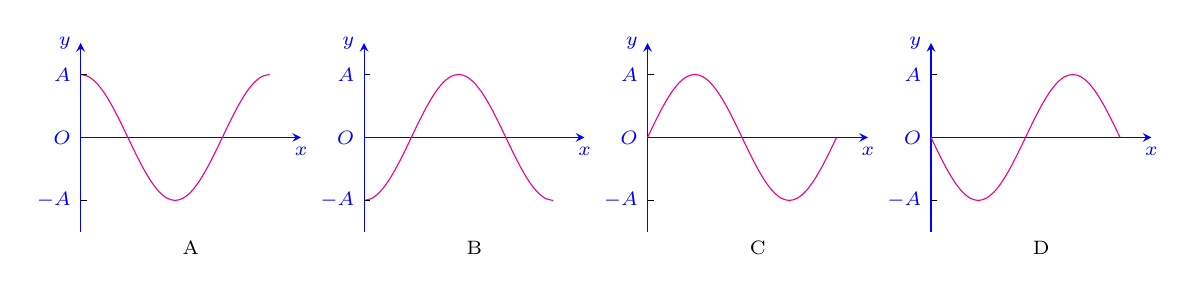
\begin{tikzpicture}[>=stealth,font=\scriptsize]
	\begin{scope}[scale=.8]
		\draw[->,blue] (0,0)node[left]{\(O\)}--(3.5,0)node[below]{\(x\)};
		\draw[->,blue] (0,-1.5)--(0,1.5)node[left]{\(y\)};
		\draw[domain=0:3,smooth,magenta] plot(\x,{cos(2*pi*\x/3 r)});
		\draw (.1,1)--(0,1)node[left,blue]{\(A\)};
		\draw (.1,-1)--(0,-1)node[left,blue]{\(-A\)};
		\node at(1.75,-1.5)[below]{ A};
	\end{scope}
	\begin{scope}[scale=.8,xshift=4.5cm]
		\draw[->,blue] (0,0)node[left]{\(O\)}--(3.5,0)node[below]{\(x\)};
		\draw[->,blue] (0,-1.5)--(0,1.5)node[left]{\(y\)};
		\draw[domain=0:3,smooth,magenta] plot(\x,{-cos(2*pi*\x/3 r)});
		\draw (.1,1)--(0,1)node[left,blue]{\(A\)};
		\draw (.1,-1)--(0,-1)node[left,blue]{\(-A\)};
		\node at(1.75,-1.5)[below]{ B};
	\end{scope}
	\begin{scope}[scale=.8,xshift=9cm]
		\draw[->,blue] (0,0)node[left]{\(O\)}--(3.5,0)node[below]{\(x\)};
		\draw[->,blue] (0,-1.5)--(0,1.5)node[left]{\(y\)};
		\draw[domain=0:3,smooth,magenta] plot(\x,{sin(2*pi*\x/3 r)});
		\draw (.1,1)--(0,1)node[left,blue]{\(A\)};
		\draw (.1,-1)--(0,-1)node[left,blue]{\(-A\)};
		\node at(1.75,-1.5)[below]{ C};
	\end{scope}
	\begin{scope}[scale=.8,xshift=13.5cm]
		\draw[->,blue] (0,0)node[left]{\(O\)}--(3.5,0)node[below]{\(x\)};
		\draw[->,blue] (0,-1.5)--(0,1.5)node[left]{\(y\)};
		\draw[domain=0:3,smooth,magenta] plot(\x,{-sin(2*pi*\x/3 r)});
		\draw (.1,1)--(0,1)node[left,blue]{\(A\)};
		\draw (.1,-1)--(0,-1)node[left,blue]{\(-A\)};
		\node at(1.75,-1.5)[below]{ D};
	\end{scope}
\end{tikzpicture}
\begin{answer}
    D
\end{answer}